\section{Conclusion}

{\begin{center}
    \textcolor{red}{\Huge{THIS IS A SAMPLE SECTION}}  % Remove or comment out this line.
\end{center}

Conclusion

{\textcolor{blue}{This section exhibits usefull \LaTeX\ packages relevant for Noroff year 1 course.}}

\section{Code snippet sample}

\subsection{Stylized Code Typesetting Sample}

\insertcode{tex/hello_world.py}{This is "Hello World" in Python}

Every code tutorial has a "Hello World"!

\insertcode{tex/TestCode.py}{This is another Python code}

This is the conclusion page with a code listing.

\section{TiKZ package}

\subsection{TiKZ package - Graph and illustration Sample}

A very simple use of TiKZ package.

\begin{tikzpicture}
    \draw(-1.5,0)-- (1.5,0);
    \draw(0,-1.5)-- (0,1.5);
\end{tikzpicture}

Source: \url{https://ctan.uib.no/graphics/pgf/base/doc/pgfmanual.pdf}

\subsection{TiKZ package - Drawing Sample}

A drawing with TiKZ

\begin{figure}[H]
    \begin{center}
      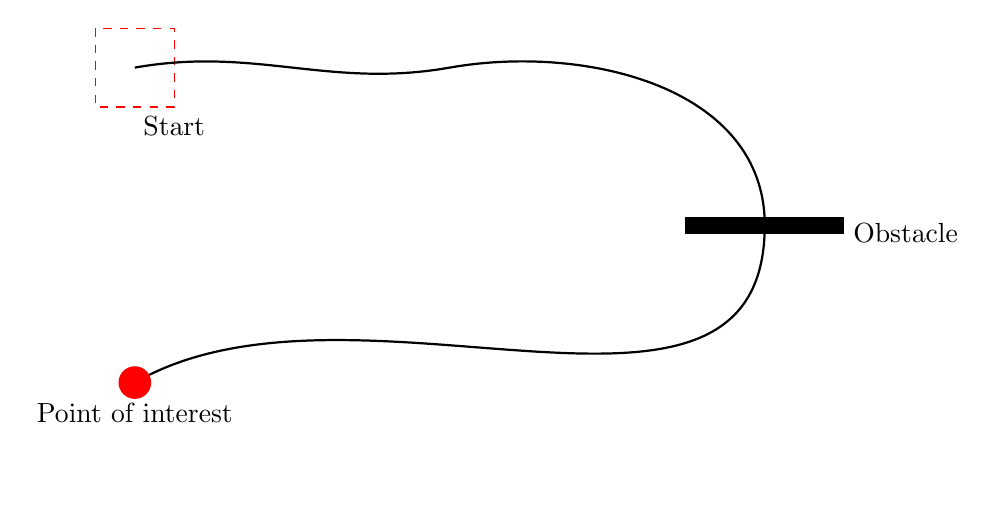
\begin{tikzpicture}
        \draw [red,dashed] (-2.5,2.5) rectangle (-1.5,1.5) node [black,below] {Start}; % Draws a rectangle
        \draw [thick] (-2,2) % Draws a line
        to [out=10,in=190] (2,2)
        to [out=10,in=90] (6,0) 
        to [out=-90,in=30] (-2,-2);    
        \draw [fill] (5,0.1) rectangle (7,-0.1) node [black,right] {Obstacle}; % Draws another rectangle
        \draw [red,fill] (-2,-2) circle [radius=0.2] node [black,below=4] {Point of interest}; % Draws a circle
      \end{tikzpicture}
      \caption{An example graphic made with tikz.}
    \end{center}
\end{figure}

Source: \url{https://www.latex-tutorial.com/tutorials/tikz/}

\subsection{TiKZ package - Venn diagram Sample}

A venn diagram with TiKZ

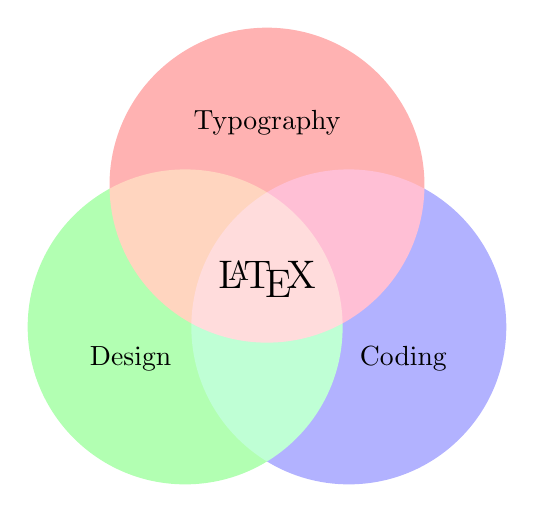
\begin{tikzpicture}
    \begin{scope}[blend group = soft light]
      \fill[red!30!white]   ( 90:1.2) circle (2);
      \fill[green!30!white] (210:1.2) circle (2);
      \fill[blue!30!white]  (330:1.2) circle (2);
    \end{scope}
    \node at ( 90:2)    {Typography};
    \node at ( 210:2)   {Design};
    \node at ( 330:2)   {Coding};
    \node [font=\Large] {\LaTeX};
\end{tikzpicture}

Source: \url{https://texample.net/tikz/examples/venn/}

\section{PlantUML .png in \LaTeX}

\begin{figure}[H]
  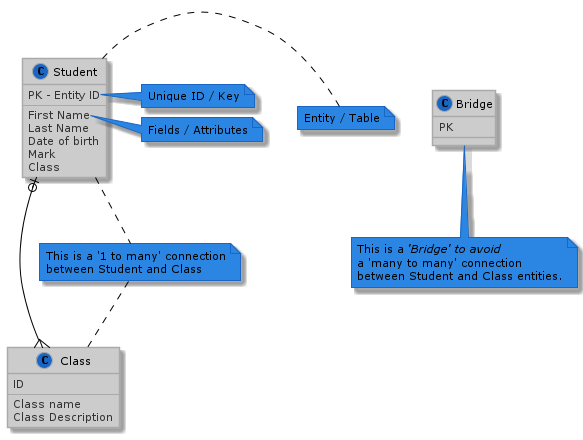
\includegraphics[width=500pt]{out/uml/SampleUML/SampleERD.png}
  \caption{Sample ERD .png}
  \label{fig:Sample ERD as .png}
\end{figure}

\begin{figure}[H]
  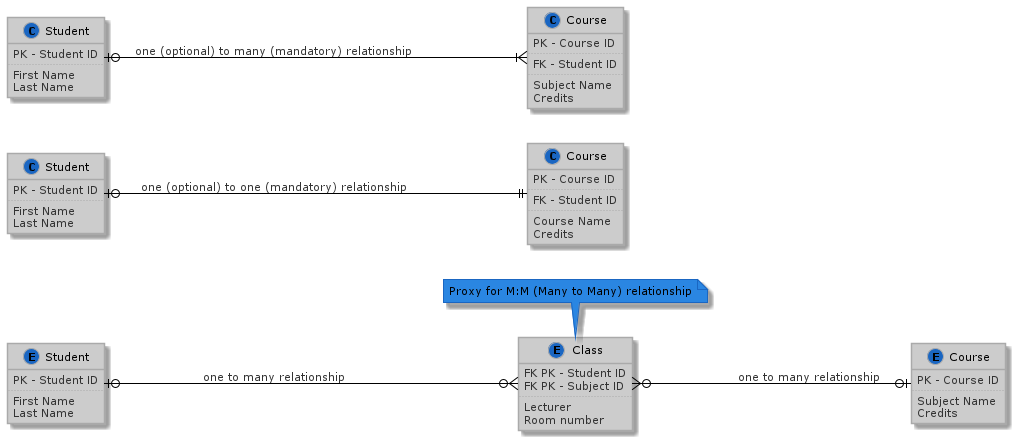
\includegraphics[width=500pt]{out/ERD_Sample_2.png}
  \caption{Sample ERD .png}
  \label{fig:Sample ERD as .png}
\end{figure}

\section{Custom Environments}

\begin{followup}[Search for...]
  Query something...
\end{followup}

\begin{notes}[Notes title]
  This is a note.
\end{notes}

\begin{question}[What is]
  This is a question.
\end{question}

\section{Image Positioning}

Sample of pictures positioned side by side

\begin{figure}[h]
  \begin{subfigure}{0.5\textwidth}
      \centering
          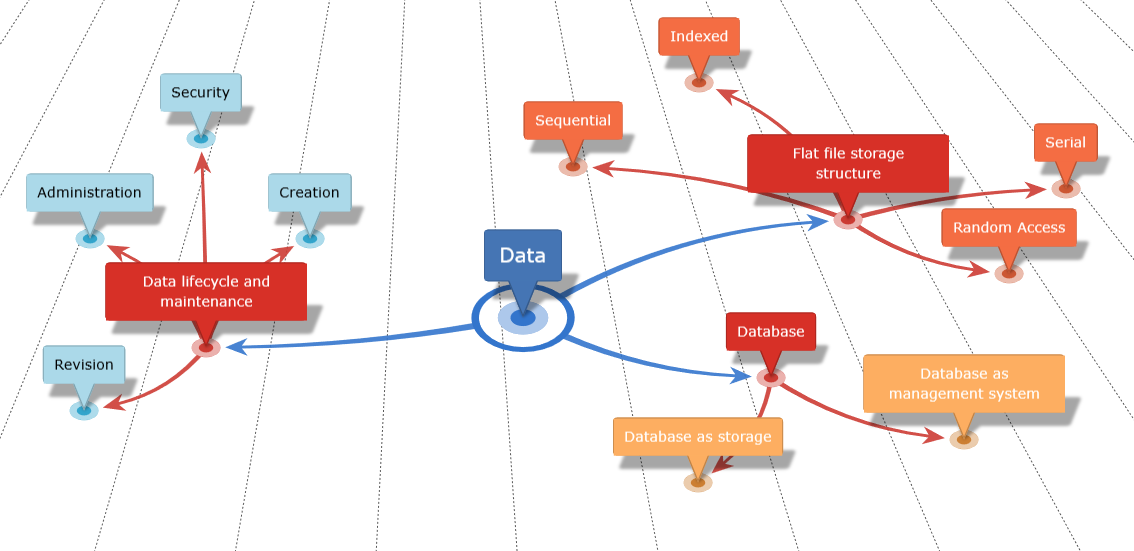
\includegraphics[width=0.95\textwidth]{tex/Data_cropped.png}
              \caption{Image 1}
              \label{fig:Task2_pic01}    
  \end{subfigure}
  \begin{subfigure}{0.5\textwidth}
      \centering
          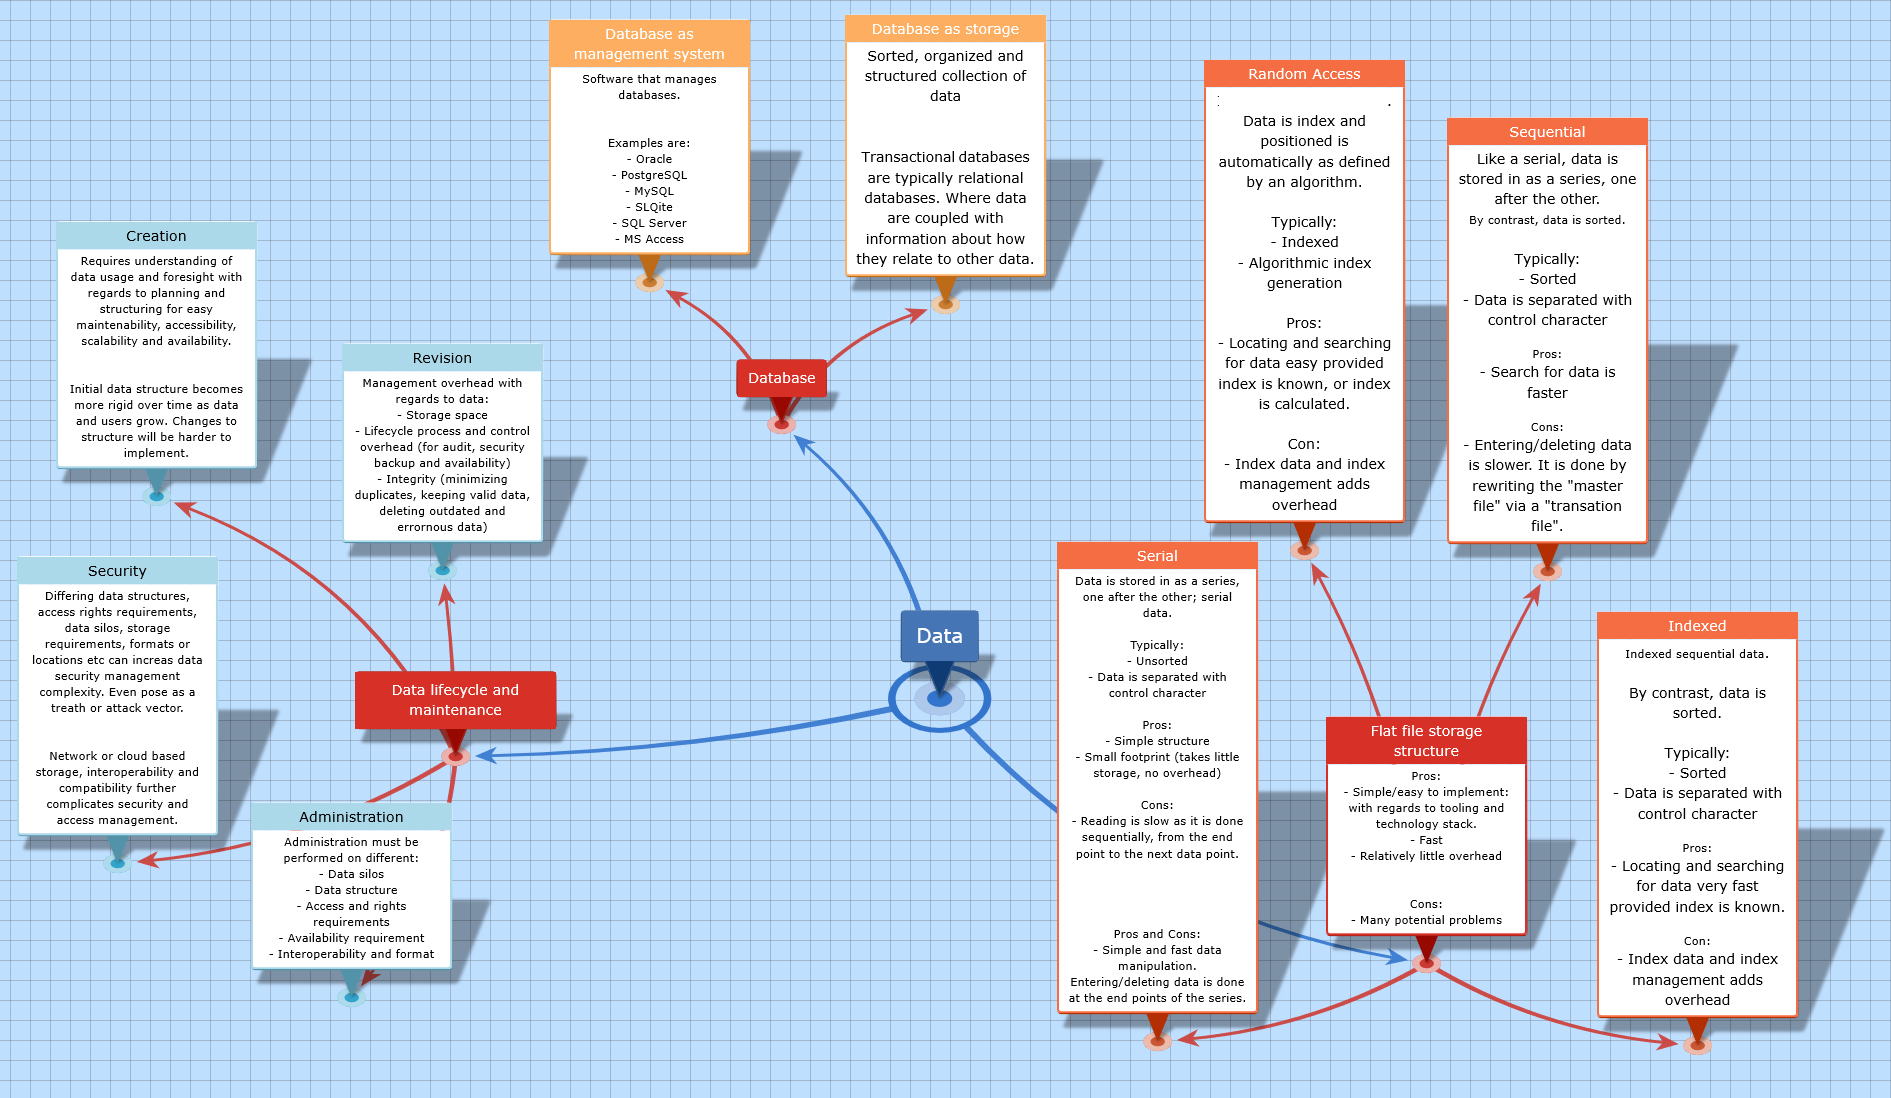
\includegraphics[width=0.95\textwidth]{tex/Data_cropped2.png}
              \caption{Image 2}
              \label{fig:Task2_pic04}
  \end{subfigure}

  \begin{subfigure}{0.5\textwidth}
    \centering
        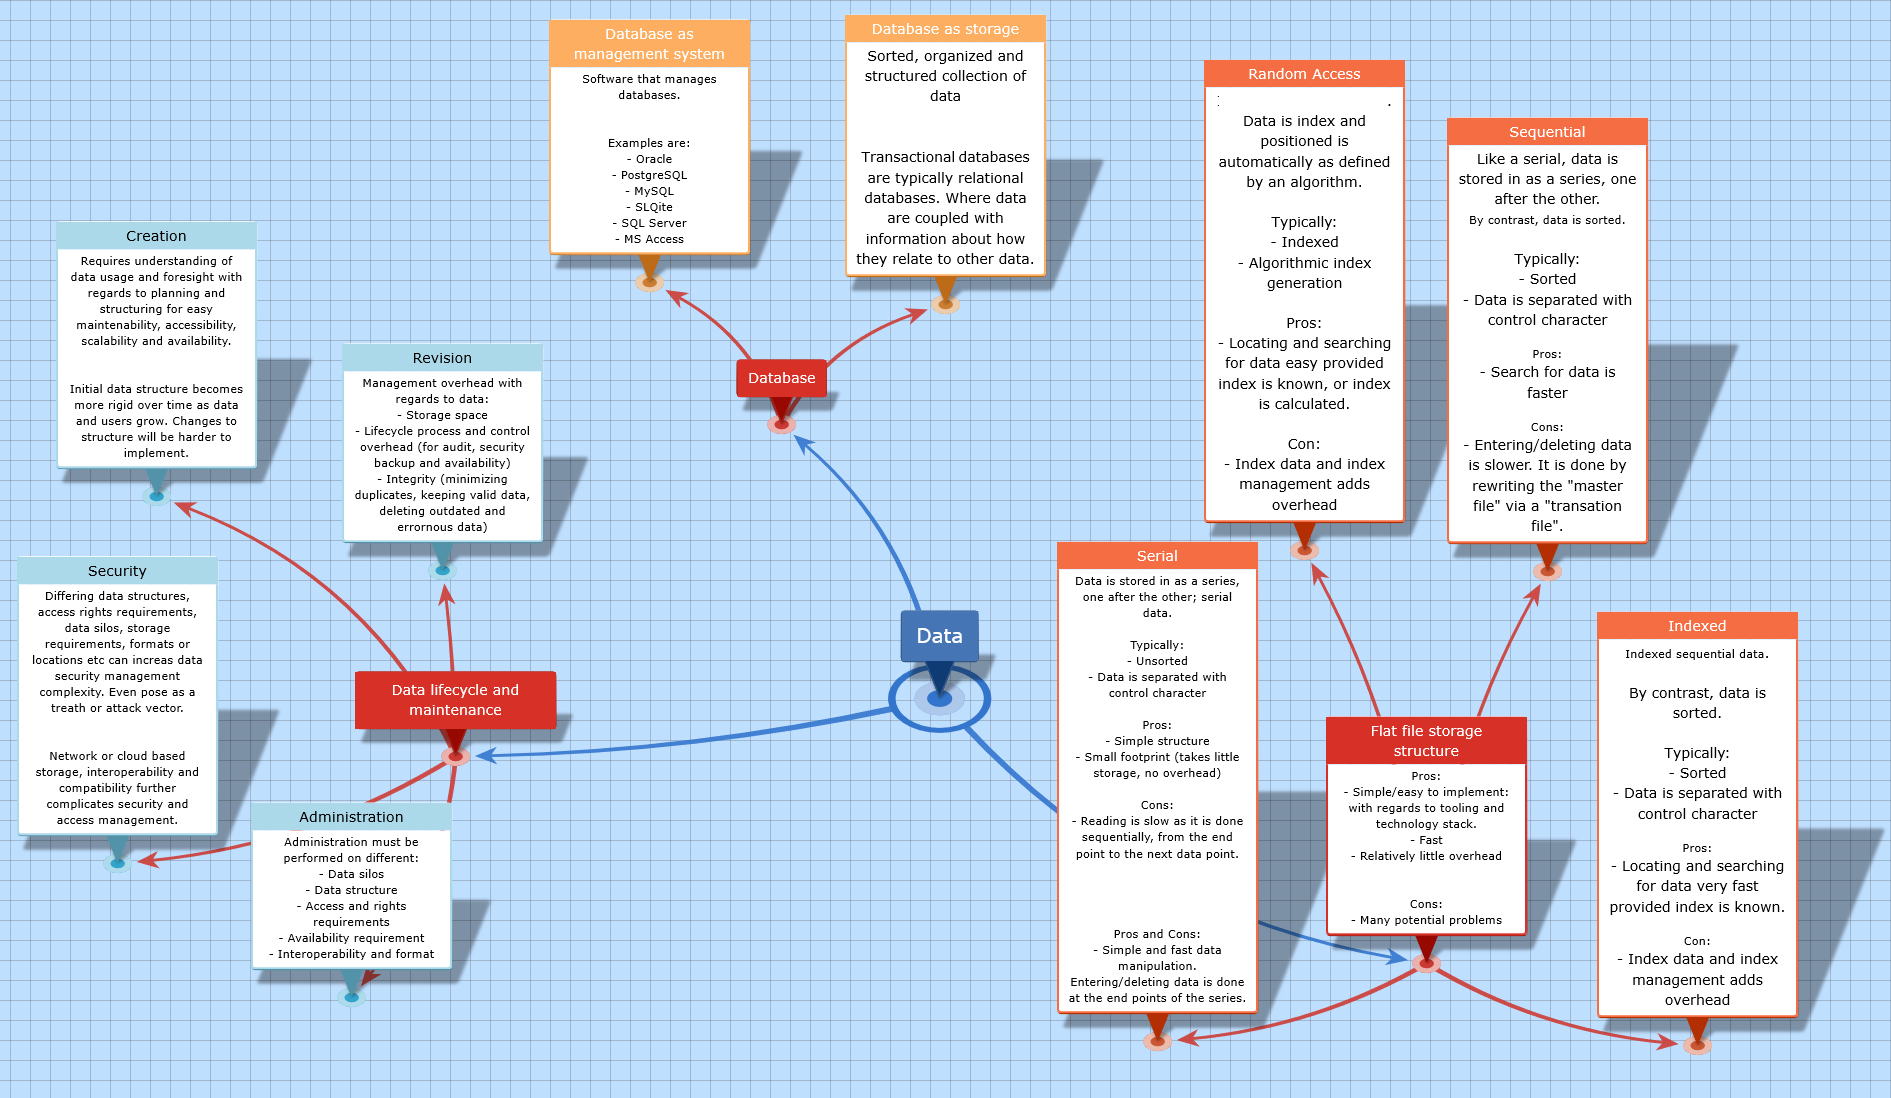
\includegraphics[width=0.95\textwidth]{tex/Data_cropped2.png}
            \caption{Image 2}
            \label{fig:Task2_pic04}
  \end{subfigure}
  \begin{subfigure}{0.5\textwidth}
    \centering
        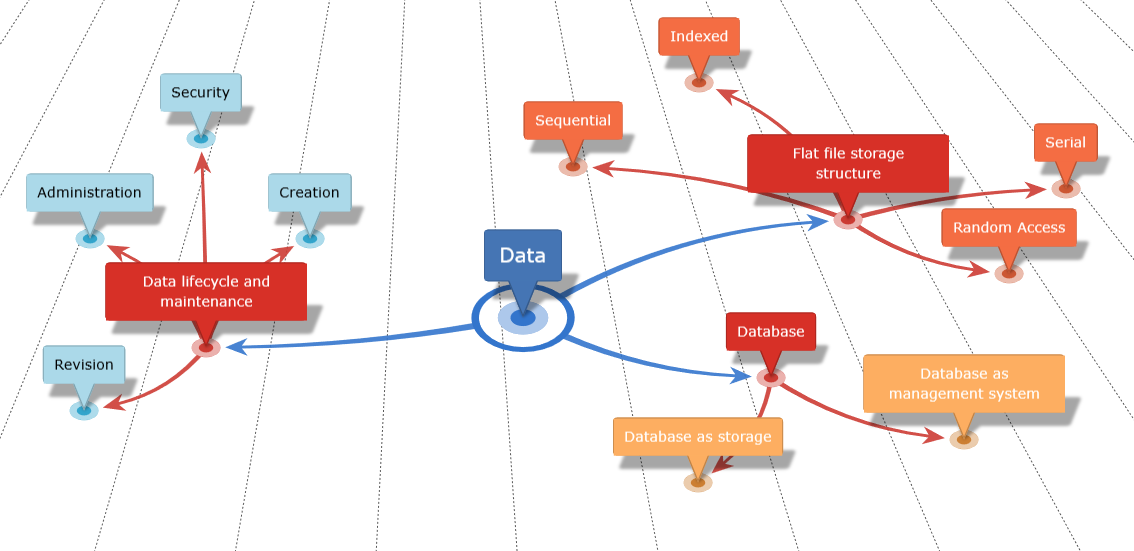
\includegraphics[width=0.95\textwidth]{tex/Data_cropped.png}
            \caption{Image 1}
            \label{fig:Task2_pic01}    
\end{subfigure}

  \caption{images 1 and 2 are order flipped to images 2 and 1}
  \label{fig:Task2_pic03}
\end{figure}



\section{Bibliography and Citation Sample}


You site a source by referring to a source in the .bib file.

This information is cited from an article from \cite{Richardson2020a, GangBoard2019}. 2'nd citation is from \cite{Williams2020}.

This is a citation number 1 \cite{Kim2018a}. Then comes citation number 2 \cite{Politou2018b}. 